\documentclass[margin = 0mm]{standalone}

\usepackage{cascadia-code}
\usepackage[T1]{fontenc}
\usepackage{xcolor}
\usepackage{tikz}

\renewcommand*\familydefault{\ttdefault}

\newcommand{\colorNode}[3]{
	\definecolor{tmpColor}{HTML}{#1}
	\node[below right, background, fill = tmpColor, minimum width = 1.5cm, minimum height = 0.75cm] at (#2, #3) {\MakeUppercase{#1}};
}

\newcommand{\colorNodeInv}[3]{
	\definecolor{tmpColor}{HTML}{#1}
	\node[below right, foreground, fill = tmpColor, minimum width = 1.5cm, minimum height = 0.75cm] at (#2, #3) {\MakeUppercase{#1}};
}

\definecolor{background}{HTML}{1A1416}
\definecolor{foreground}{HTML}{E9DBDF}

\begin{document}
	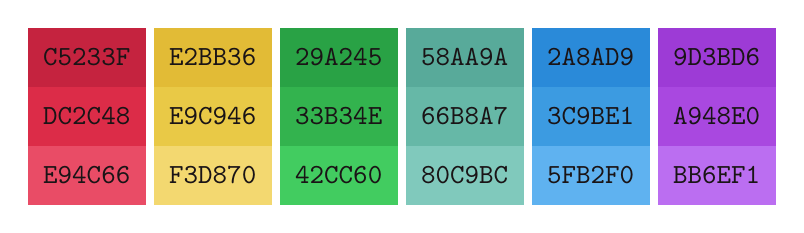
\begin{tikzpicture}%

		% reds
		\colorNode{C5233F}{0.0}{-0.50}
		\colorNode{DC2C48}{0.0}{-1.25}
		\colorNode{E94C66}{0.0}{-2.00}

		% yellows
		\colorNode{E2BB36}{1.6}{-0.50}
		\colorNode{E9C946}{1.6}{-1.25}
		\colorNode{F3D870}{1.6}{-2.00}


		% green
		\colorNode{29A245}{3.2}{-0.50}
		\colorNode{33B34E}{3.2}{-1.25}
		\colorNode{42CC60}{3.2}{-2.00}

		% cyans
		\colorNode{58AA9A}{4.8}{-0.50}
		\colorNode{66B8A7}{4.8}{-1.25}
		\colorNode{80C9BC}{4.8}{-2.00}

		% blues
		\colorNode{2A8AD9}{6.4}{-0.50}
		\colorNode{3C9BE1}{6.4}{-1.25}
		\colorNode{5FB2F0}{6.4}{-2.00}

		% purples
		\colorNode{9D3BD6}{8.0}{-0.50}
		\colorNode{A948E0}{8.0}{-1.25}
		\colorNode{BB6EF1}{8.0}{-2.00}

	\end{tikzpicture}%
\end{document}
